% Observer/Estimator
% Author: Dominik Haumann
\documentclass[landscape,a5paper,11pt]{standalone}
\usepackage[utf8x]{inputenc} % utf8 encoding
\usepackage[T1]{fontenc} % use T1 fonts
\usepackage{amsmath} % nice math symbols
\usepackage{bm} % bold math
\usepackage{color} % change text color        

\usepackage{tikz}
\usetikzlibrary{matrix} % for block alignment
\usetikzlibrary{arrows} % for arrow heads

% TikZ styles for drawing
\tikzstyle{block} = [draw,rectangle,thick,minimum height=2em,minimum width=2em]
\tikzstyle{sum} = [draw,circle,inner sep=0mm,minimum size=2mm]
\tikzstyle{connector} = [->,thick]
\tikzstyle{line} = [thick]
\tikzstyle{branch} = [circle,inner sep=0pt,minimum size=1mm,fill=black,draw=black]
\tikzstyle{guide} = []
\tikzstyle{snakeline} = [connector, decorate, decoration={pre length=0.2cm,
                         post length=0.2cm, snake, amplitude=.4mm,
                         segment length=2mm},thick, magenta, ->]

\renewcommand{\vec}[1]{\ensuremath{\boldsymbol{#1}}} % bold vectors
\def \myneq {\skew{-2}\not =} % \neq alone skews the dash

\begin{document}
  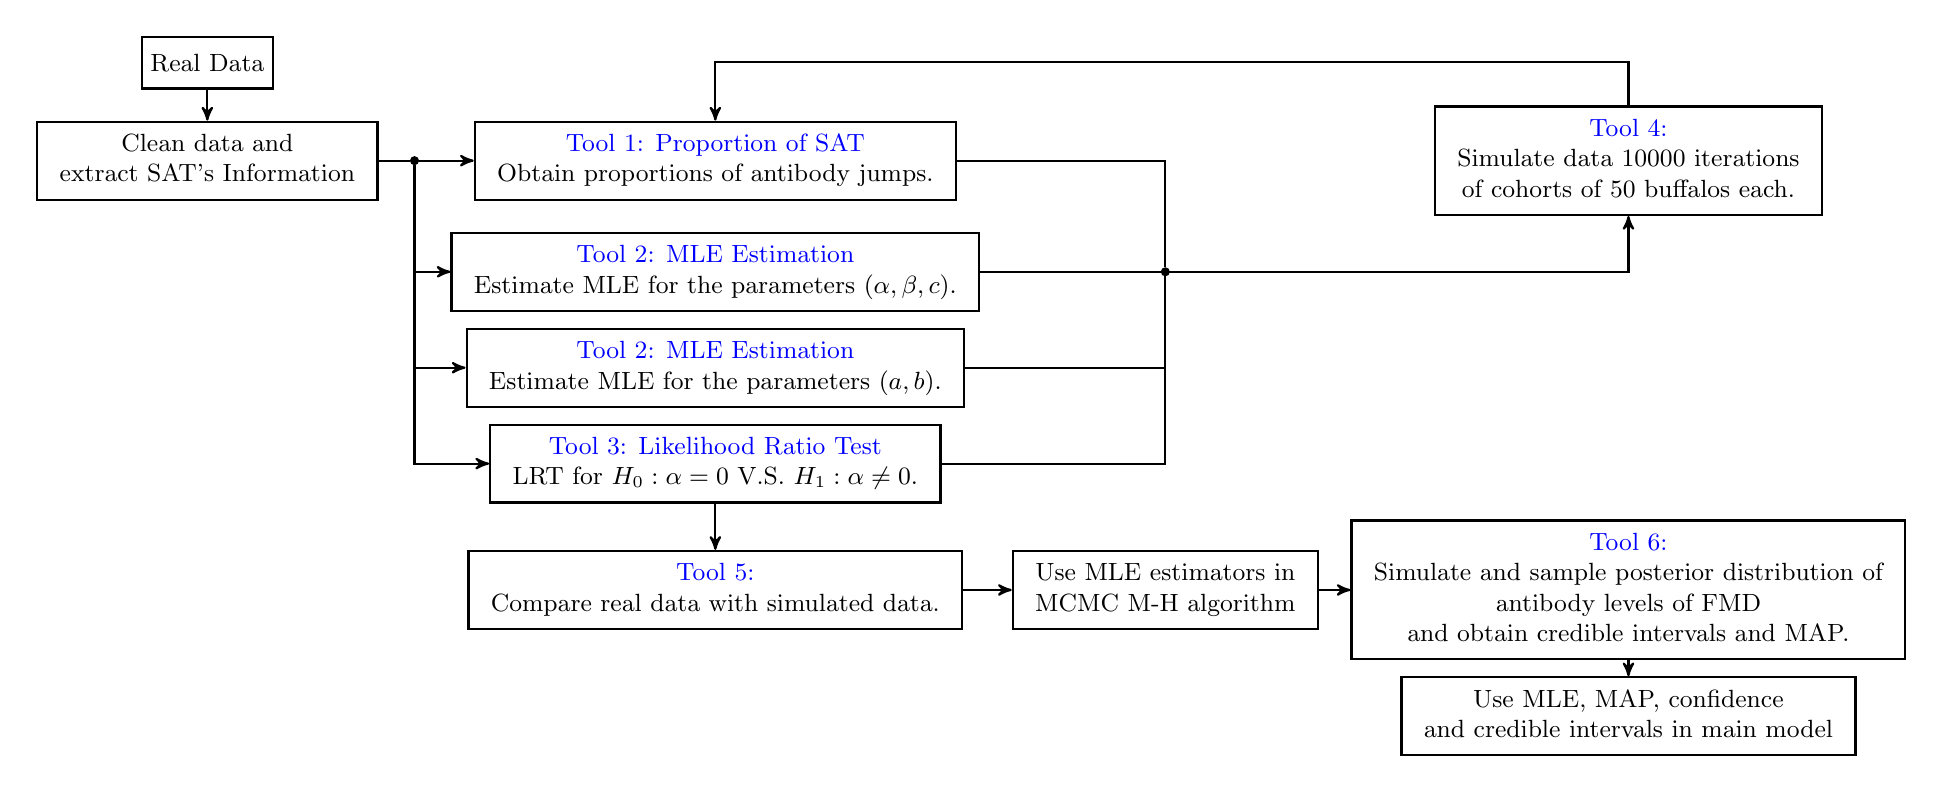
\begin{tikzpicture}[scale=1, auto, >=stealth']
    \small
    % node placement with matrix library: 5x4 array
    \matrix[ampersand replacement=\&, row sep=0.2cm, column sep=0.4cm] {
      %
			\node[block] (data) {$\mbox{Real Data}$}; \&  \& \&\&\\
			\node[block] (data1) {$\begin{array}{c}\mbox{Clean data and}\\ 
			\mbox{extract SAT's Information}
			\end{array}$}; \& 
			\node[branch] (u1) {};\&  
			\node[block] (tool1) {$\begin{array}{c}\mbox{\color[rgb]{0,0,1} Tool 1: Proportion 
			of SAT}\\
			\mbox{Obtain proportions of antibody jumps.}\end{array}$};\& \&
			\node[block] (tool4) {$\begin{array}{c}\mbox{\color[rgb]{0,0,1} Tool 4:}\\
			\mbox{Simulate data 10000 iterations}\\ \mbox{of cohorts of 50 buffalos each.}
			\end{array}$};\\
			\&  \&
			\node[block] (tool2a) {$\begin{array}{c}\mbox{\color[rgb]{0,0,1} Tool 2: MLE Estimation}\\
			\mbox{Estimate MLE for the parameters $(\alpha,\beta,c)$.}\end{array}$}; \&
			\node[branch] (u2) {};\&\\
			\&  \&\node[block] (tool2b) {$\begin{array}{c}\mbox{\color[rgb]{0,0,1} Tool 2: MLE Estimation}\\
			\mbox{Estimate MLE for the parameters $(a,b)$.}\end{array}$}; \&\&\\
			\&  \&
			\node[block] (tool3) {$\begin{array}{c}\mbox{\color[rgb]{0,0,1} Tool 3: Likelihood Ratio Test}\\
			\mbox{LRT for $H_0:\alpha=0$ V.S. $H_1:\alpha\neq0$.}\end{array}$}; \&\&\\
			\&  \&
			\node[block] (tool5) {$\begin{array}{c}\mbox{\color[rgb]{0,0,1} Tool 5:}\\ \mbox{Compare real data with 
			simulated data.}\end{array}$}; \&
			\node[block] (step) {$\begin{array}{c}\mbox{Use MLE estimators in}\\
			\mbox{MCMC M-H algorithm}\end{array}$};\&
			\node[block] (tool6) {$\begin{array}{c}\mbox{\color[rgb]{0,0,1} Tool 6:}\\ 
			\mbox{Simulate and sample posterior distribution of}\\ \mbox{antibody levels 
			of FMD}\\ \mbox{and obtain credible intervals and MAP.}\end{array}$};\\
			\&  \& \&\&\node[block] (final) {$\begin{array}{c}\mbox{Use MLE, MAP, confidence}\\ 
			\mbox{and credible intervals 
			in main model}\end{array}$};\\
			};
			% now link the nodes
			\draw [connector] (data) -- (data1);
			\draw [line] (data1) -- (u1);
			\draw [connector] (u1) |- (tool1);
			\draw [connector] (u1) |- (tool2a);
			\draw [connector] (u1) |- (tool2b);
			\draw [connector] (u1) |- (tool3);
			\draw [line] (tool1) -| (u2);
			\draw [line] (tool2a) -| (u2);
			\draw [line] (tool2b) -| (u2);
			\draw [line] (tool3) -| (u2);
			\draw [connector] (u2) --++(0,0cm)-| (tool4);
			\draw [connector] (tool4) |-++(0,.75cm) --++(0,.5cm)-| (tool1);
			\draw [connector] (tool3) -- (tool5);
			\draw [connector] (tool5) -- (step);
			\draw [connector] (step) -- (tool6);
			\draw [connector] (tool6) -- (final);
    %\draw [connector] (f1) -| node[near end] {$\vec{y}_i$} (e1);
    %\draw [connector] (e1) -- (L1);
    %\draw [connector] (L1) -| (v1);
    %\draw [connector] (v1) -- node {$\vec{v}_i$} (o1);
    %\draw [connector] (u1) |- (v1);
    %\draw [connector] (o1) -| node[pos=0.96] {$-$} node [near end, swap]
                      %{$\widetilde{\vec{y}}_i$} (e1);
    %\draw [connector] (o1.south) -- ++(0,-.5cm) -| node [near start]
                      %{$\widetilde{\vec{x}}_i$} ($(F1.south) + (0.4cm, 0em)$);
    %
    %
			%
      %\node[block] (F1) {$\vec{u}_i = F_i(\{\widetilde{\vec{x}}_j\}_{j=1}^N)$}; \&
      %\node[branch] (u1) {}; \&
      %\&
      %\node[block] (f1) {$\begin{matrix}
            %\dot{\vec{x}}_i =
              %f_i(\vec{x}_i,
                  %\textcolor{red}{\{\widetilde{\vec{x}}_j\}_{j \myneq i}},
                  %\vec{u}_i,
                  %t)\\
            %\vec{y}_i =
              %g_i(\vec{x}_i,
                  %\textcolor{blue}{\{\widetilde{\vec{x}}_j\}_{j \myneq i}},
                  %t)
          %\end{matrix}$}; \& \\
%
      %\&
      %\&
      %\&
      %\node[block] (L1) {$\vec{e}_i(\vec{y}_i - \widetilde{\vec{y}}_i)$};\&
      %\node [sum] (e1) {}; \\
%
      %\&
      %\&
      %\node[sum] (v1) {}; \&
      %\node[block] (o1) {$\begin{matrix}
            %\dot{\widetilde{\vec{x}}}_i =
              %\widetilde{f}_i(\widetilde{\vec{x}}_i,
                              %\textcolor{red}{\{\widetilde{\vec{x}}_j\}_{j \myneq i}},
                              %\vec{v}_i, t)\\
              %\widetilde{\vec{y}}_i =
                %g_i(\widetilde{\vec{x}}_i,
                    %\textcolor{blue}{\{\widetilde{\vec{x}}_j\}_{j \myneq i}},
                    %t)
          %\end{matrix}$};
      %\&
      %\\
      %\node[guide] (i1) {}; \& \& \& \& \\
    %};
%
    %% now link the nodes
    %\draw [line] (F1) -- (u1);
    %\draw [connector] (u1) -- node {$u_i$} (f1);
    %\draw [connector] (f1) -| node[near end] {$\vec{y}_i$} (e1);
    %\draw [connector] (e1) -- (L1);
    %\draw [connector] (L1) -| (v1);
    %\draw [connector] (v1) -- node {$\vec{v}_i$} (o1);
    %\draw [connector] (u1) |- (v1);
    %\draw [connector] (o1) -| node[pos=0.96] {$-$} node [near end, swap]
                      %{$\widetilde{\vec{y}}_i$} (e1);
    %\draw [connector] (o1.south) -- ++(0,-.5cm) -| node [near start]
                      %{$\widetilde{\vec{x}}_i$} ($(F1.south) + (0.4cm, 0em)$);
    %
    %% draw the snake lines with offset (using the calc library)
    %\draw [snakeline] ($(i1) - (0.4cm, -1cm)$) -- node
      %{$\{\widetilde{\vec{x}}_j\}_{j \myneq i}$} ($(F1.south) - (0.4cm, 0em)$);
%
    %\draw [snakeline, swap] ($(v1.east) - (1.0cm, 0.4cm)$) -- node
      %{$\{\widetilde{\vec{x}}_j\}_{j \myneq i}$} ($(o1.west) - (0cm, 0.4cm)$);
    %
    %\draw [snakeline, swap] ($(u1.east) + (0.1cm, -0.4cm)$) -- node
      %{$\{\widetilde{\vec{x}}_j\}_{j \myneq i}$} ($(f1.west) - (0cm, 0.4cm)$);

  \end{tikzpicture}

\end{document}